\documentclass[twoside]{article}

\usepackage{ustj}

\usepackage{tikz}
\usepackage{pgfplots}
\pgfplotsset{compat=1.10}
\usetikzlibrary{shapes.geometric,arrows,fit,matrix,positioning}
\tikzset
{
    treenode/.style = {circle, draw=black, align=center, minimum size=1cm},
    subtree/.style  = {circle, draw=darkgray, dashed, text=darkgray, align=center, minimum size=1cm}
}

\setcounter{tocdepth}{2}

\addbibresource{mss.bib}

\newcommand{\authorname}{Tim Galebach}
\newcommand{\authorpatp}{\patp{timluc-miptev}}
\newcommand{\affiliation}{Uncentered Systems}

%  Make first page footer:
\fancypagestyle{firststyle}{%
\fancyhf{}% Clear header/footer
\fancyhead{}
\fancyfoot[L]{{\footnotesize
              %% We toggle between these:
              % Manuscript submitted for review.\\
              {\it Urbit Systems Technical Journal} II:1 (2025):  1–46. \\
              ~ \\
              Address author correspondence to \authorpatp.
              }}
}
%  Arrange subsequent pages:
\fancyhf{}
\fancyhead[LE]{{\urbitfont Urbit Systems Technical Journal}}
\fancyhead[RO]{Nock for Everyday Coders}
\fancyfoot[LE,RO]{\thepage}

%%MANUSCRIPT
\title{Nock for Everyday Coders}
\author{\authorname~\authorpatp \\ \affiliation}
\date{}

\begin{document}

\maketitle
\thispagestyle{firststyle}

\begin{abstract}
  Nock is not super complex, and most programmers can learn the basics of it rapidly. The mental model gained by learning Nock turns out to be very useful in learning Hoon and understanding Urbit.
  While the Urbit docs generally suggest to not worry about Nock, Nock is very simple and small.  Most programmers will feel more comfortable in Hoon having learned Nock's basics.
  The goal of this tutorial is to explain Nock clearly in terms most programmers will relate to, to impart a feeling of confidence with very basic Nock, and to give a knowledge of Nock’s idioms and big ``wins" so that they carry over to learning Hoon.
  This tutorial was originally published online by \patp{timluc-miptev} in early 2020 and remains an excellent exposition of Nock's affordances.
\end{abstract}

% We will adjust page numbering in final editing.
\pagenumbering{arabic}
\setcounter{page}{1}

\tableofcontents

\section{Getting Started}

When people first look at Nock, they see the definition, which is fairly intimidating.  I'm talking about lines like this:

\begin{lstlisting}[style=listingcode]
/[(a + a) b]        /[2 /[a b]]
\end{lstlisting}

The problem is, the programmer may already know that Nock code looks more like the below – just lists of numbers, with no symbols:

\begin{lstlisting}[style=listingcode]
[6
 [5 [0 6] [1 0]]
 [0 7]
 [9 4 [[0 2] [2 [0 6] [0 5]] [4 0 7]]]
]
\end{lstlisting}

What gives? Which one is the ``real'' Nock?

\subsection{Phases of Nock}

We are looking at two different things in the examples above:

\begin{enumerate}
  \item  Pseudocode for \emph{how to interpret} Nock.
  \item  Code to be interpreted (written as lists of numbers).
\end{enumerate}

The symbols and spec are pseudocode, not real Nock code. They could just as easily be written in English, and they will never be written down as actual Nock code and given to an interpreter. They represent what an interpreter should do to turn Nock code into interpreter instructions.

The lists of numbers are the actual Nock code. This is what you feed to an interpreter to get some result.

\subsection{What Is a Nock Interpreter?}

An interpreter can be a computer program, or it can be a human manually expanding Nock code into results. In both cases, the program and human have to know the Nock pseudocode in order to do the right thing with incoming Nock code.

So a Nock interpreter is any entity that takes Nock code as input, and gives a noun as output. A noun can be:

\begin{lstlisting}[style=listingcode]
:: a number
782
:: a cell (pair with two elements)
[782 9872]
:: each element can itself be a pair
[782 [9872 89728]]
:: the above can be written as
[782 9872 89728]
\end{lstlisting}

\subsection{How to Run Nock Code}

We will be expanding Nock pseudocode manually in the examples that follow, in effect acting as our own interpreter.

If we want to check that we're getting the right results from our manual interpretation, we need to run a Nock interpreter, such as the Urbit Dojo.

\begin{enumerate}
  \item  Start up a Dojo session on a fake ship.\footnote{Consult \texttt{docs.urbit.org} for details.}
  \item  At the prompt, we can execute Nock using \texttt{.*} dottar, e.g., \lstinline[style=inlinecode]{.*(NOCK_SUBJECT, NOCK_FORMULA)}.
\end{enumerate}

\subsection{Subject, Formula?}

Let's keep this simple:

\begin{itemize}
  \item  subject = an argument to a function
  \item  formula = the function
\end{itemize}

That's it. We'll see below how this works, going really slowly with examples.

\subsection{Evaluating Our First Nock Code}

OK, so the interpreter takes two arguments, a ``subject" and a ``formula". Both are nouns (a number or a cell). Let's run some insanely simple Nock code in the Dojo:\footnote{Code samples beginning with \lstinline[style=inlinecode]{>} are Dojo inputs (to wit, Hoon expressions).}

\begin{lstlisting}[style=listingcode]
> .*(42 [0 1])
42
\end{lstlisting}

In the above, \lstinline[style=inlinecode]{42} is our subject. \lstinline[style=inlinecode]{[0 1]} is our formula.

Formulas are always cells, and the first element of the cell is a number that you can think of as \emph{the name of the function}.

In this case, our function name is \lstinline[style=inlinecode]{0}, which is the memory slot function. It is always followed by 1 number, in this case \lstinline[style=inlinecode]{1}, which is the number of the memory slot to fetch in the subject.

Whenever we look at Nock code, we want to ask:

\begin{itemize}
  \item  What is the subject (function argument)? In this case, it's \lstinline[style=inlinecode]{42}.
  \item  What is the formula (function)? In this case, it's \lstinline[style=inlinecode]{[0 1]}.
  \item  What value does that formula (function) produce when called on this subject (argument)? In this case, the return value is \lstinline[style=inlinecode]{42}.
\end{itemize}

Why is the return value \lstinline[style=inlinecode]{42}? How does this formula work?

\section{Fundamental Opcodes}

\subsection{Nock's Simplest Functions, \lstinline[style=inlinecode]{0} and \lstinline[style=inlinecode]{1}}

The two most basic Nock functions are \lstinline[style=inlinecode]{0} address and \lstinline[style=inlinecode]{1} constant. The goal here is to get strong intuitions of what they do, how they handle edge cases, and how this relates to the Nock spec/pseudocode.

\subsection{Binary Tree Addressing}

Before getting started on Nock proper, we should understand how Nock and Hoon handle addresses in binary trees.  If you already understand why memory slot 5 of \lstinline[style=inlinecode]{[['apple' %pie] [0b1101 0xdad]]} is \lstinline[style=inlinecode]{%pie}, you are good to go and can skip ahead to the Section~\ref{sxn:nock0}.

Every noun in Nock can be thought of as a tree, which means we can give an exact number to access any position in the tree. This means that, no matter how big our subject (argument) is, we can yank a value out of any part of it.

Noun tree addressing is directly addressed in the Nock specification:

\begin{lstlisting}[style=listingcode]
/[1 a]              a
/[2 a b]            a
/[3 a b]            b
/[(a + a) b]        /[2 /[a b]]
/[(a + a + 1) b]    /[3 /[a b]]
\end{lstlisting}

\noindent{}
This permits the address to be defined within a particular subtree as well as within the overall tree (Figure \ref{fig:treefull}).

\begin{figure}[hbt!]
  \centering
  \caption{A binary tree with labeled node addresses to several layers. \label{fig:treefull}}
  {
    \begin{tikzpicture}
    [->,>=stealth',level 1/.style={sibling distance = 8cm/#1, level distance = 1.5cm},level 2/.style={sibling distance = 4cm/#1, level distance = 1.5cm},level 3/.style={sibling distance = 2cm/#1, level distance = 1.5cm},level 4/.style={sibling distance = 1cm/#1, level distance = 1.5cm},scale=0.6, transform shape]
    \node [subtree] {\Large 1}
    child {
      node [subtree] {\Large 2} 
      child {
        node [subtree] {\Large 4} 
        child {
          node [subtree] {\Large 8} 
          child {
            node [treenode] {\Large 16} 
            }
          child {
            node [treenode] {\Large 17} 
          }
          }
        child {
          node [subtree] {\Large 9} 
          child {
            node [treenode] {\Large 18} 
          }
          child {
            node [treenode] {\Large 19} 
          }
          }
          }
      child {
        node [subtree] {\Large 5} 
        child {
          node [subtree] {\Large 10} 
          child {
            node [treenode] {\Large 20} 
          }
          child {
            node [treenode] {\Large 21} 
          }
        }
        child {
          node [subtree] {\Large 11} 
          child {
            node [treenode] {\Large 22} 
          }
          child {
            node [treenode] {\Large 23} 
          }
        }
          }
    }
    child {
      node [subtree] {\Large 3} 
      child {
        node [subtree] {\Large 6} 
        child {
          node [subtree] {\Large 12} 
          child {
            node [treenode] {\Large 24} 
          }
          child {
            node [treenode] {\Large 25} 
          }
        }
        child {
          node [subtree] {\Large 13} 
          child {
            node [treenode] {\Large 26} 
          }
          child {
            node [treenode] {\Large 26} 
          }
        }
    }
      child {
        node [subtree] {\Large 7} 
        child {
          node [subtree] {\Large 14} 
          child {
            node [treenode] {\Large 28} 
          }
          child {
            node [treenode] {\Large 29} 
          }
        }
        child {
          node [subtree] {\Large 15} 
          child {
            node [treenode] {\Large 30} 
          }
          child {
            node [treenode] {\Large 31} 
          }
        }
      }
    }
    ;
    \end{tikzpicture}
  }
\end{figure}

That is, how do you say which slot number you want from a given tree?  We say that:

\begin{itemize}
  \item The tree root is address 1.
  \item The head of every node $n$ is $2n$.
  \item The tail of every node $n$ is $2n+1$.
\end{itemize}

Let's take an example tree to illustrate. In Nock cell form, the tree is:

\begin{lstlisting}[style=listingcode]
[[4 5] [6 14 15]]
\end{lstlisting}

Diagrammatically, the tree looks like Figure \ref{fig:tree45}.

\begin{figure}[t]
  \centering
  \caption{A binary tree with some labeled node addresses. \label{fig:tree45}}
  {
    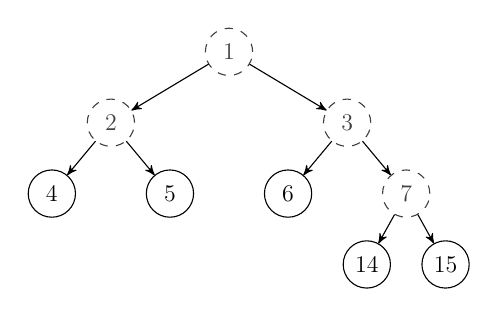
\begin{tikzpicture}
    [->,>=stealth',level/.style={sibling distance = 5cm/#1, level distance = 1.5cm},scale=0.6, transform shape]
    \node [subtree] {\Large 1}
    child {
      node [subtree] {\Large 2} 
      child {
        node [treenode] {\Large 4} 
      }
      child {
        node [treenode] {\Large 5} 
      }
    }
    child {
      node [subtree] {\Large 3} 
      child {
        node [treenode] {\Large 6} 
      }
      child {
        node [subtree] {\Large 7} 
        child {
          node [treenode] {\Large 14} 
        }
        child {
          node [treenode] {\Large 15} 
        }
      }
    }
    ;
    \end{tikzpicture}
  }
\end{figure}

\begin{itemize}
  \item  1 is the address of the whole tree, \lstinline[style=inlinecode]{[[4 5] [6 14 15]]}.
  \item  2 is the address of the left branch, \lstinline[style=inlinecode]{[4 5]}.
  \item  3 is the address of the right branch, \lstinline[style=inlinecode]{[6 14 15]}.
  \item  15 is the value \lstinline[style=inlinecode]{15}.
\end{itemize}

Let's play around now in the Dojo Nock interpreter so that we can confirm this. In each example, our subject (argument) will be the tree \lstinline[style=inlinecode]{[[4 5] [6 14 15]]}.

\begin{lstlisting}[style=listingcode]
:: formula (function) [0 1]: get the whole tree
> .*([[4 5] [6 14 15]] [0 1])
[[4 5] 6 14 15]

:: formula (function) [0 2]: get the left branch
> .*([[4 5] [6 14 15]] [0 2])
[4 5]

:: formula (function) [0 7]: get the subtree in slot 7
> .*([[4 5] [6 14 15]] [0 7])
[14 15]
\end{lstlisting}

\subsection{\lstinline[style=inlinecode]{@0@}, the “Memory Slot” Function}
\label{sxn:nock0}

The pseudocode for the \lstinline[style=inlinecode]{@0@} opcode\footnote{From this point on, we will write Nock opcodes in special type so that they can be distinguished from other numbers in Nock.  This reflects Hoon practice, which marks Nock rules as constants like \lstinline[style=inlinecode]{\%0}.  While not strictly necessary, it can be helpful when learning or coding Nock to see an explicit distinction.} is as follows:

\begin{lstlisting}[style=listingcode]
*[a @0@ b]  /[b a]
\end{lstlisting}

\lstinline[style=inlinecode]{/[b a]} is pseudocode. In English, it means ``\lstinline[style=inlinecode]{a} is a binary tree. Get the memory slot numbered \lstinline[style=inlinecode]{b}.

So if \lstinline[style=inlinecode]{a} were the tree \lstinline[style=inlinecode]{[9 10]}, and \lstinline[style=inlinecode]{b} were \lstinline[style=inlinecode]{1}, we'd get the memory slot \lstinline[style=inlinecode]{1} in the tree \lstinline[style=inlinecode]{[9 10]}, which is just the tree itself.

Written in pseudocode, that's \lstinline[style=inlinecode]{/[1 [9 10]]}. We can also do \lstinline[style=inlinecode]{/[2 [9 10]]}, which grabs memory slot \lstinline[style=inlinecode]{2}, aka \lstinline[style=inlinecode]{9}.

Let's look at some examples. I've put them first in Dojo form so that you can see how they run in that interpreter, and then I show the ``human interpreter" in pseudocode below that.

\subsubsection{Example:  Retrieve the Subject}

\begin{lstlisting}[style=listingcode]
:: get memory slot 1
> .*([50 51] [@0@ 1])
[50 51]
:: PSEUDOCODE -- replaces the Dojo's () with []
*[[50 51] [@0@ 1]]
:: *[a @0@ b] -> a = [50 51], b = 1
/[1 [50 51]]
[50 51]
\end{lstlisting}

\subsubsection{Example:  Retrieve the Head of the Subject}

\begin{lstlisting}[style=listingcode]
> .*([50 51] [@0@ 2])
50
:: PSEUDOCODE -- replaces the Dojo's () with []
*[[50 51] [0 2]]
:: *[a @0@ b] -> a = [50 51], b = 2
/[2 [50 51]]
50
\end{lstlisting}

\subsubsection{Example:  A Crash}

\begin{lstlisting}[style=listingcode]
> .*([50 51] [@0@ [0 1]])
dojo: hoon expression failed
:: PSEUDOCODE
*[[50 51] [@0@ [0 1]]]
/[[0 1] [50 51]]
:: can't evaluate this--a memory slot must be a number like 2, not a cell like [0 1]
CRASH
\end{lstlisting}

\subsubsection{Summary of \lstinline[style=inlinecode]{@0@}}

\lstinline[style=inlinecode]{@0@} is everywhere in Nock, because “get something from a memory slot” really means “store stuff in a place and get it whenever I want,” which is another name for creating variables. These memory slot numbers take the place of variable names.

If you're familiar with assembly or C, they're conceptually similar to memory pointers or registers in how Nock uses them. Keep in mind though, Nock is functional/immutable, so it doesn't update memory locations: it creates copies of data structures with altered values.

We've also seen that the memory slot function can't take just anything as the memory slot to fetch: it must receive an atom (number).

\subsection{\lstinline[style=inlinecode]{@1@}, the “Quoter” Function}
\label{sxn:nock1}

This is another really simple function. You can think of it as a “quoter”: it just returns any value passed to it exactly as it is. It ignores the subject, and just quotes the value after it. Let's look at a couple examples.

\begin{lstlisting}[style=listingcode]
> .*([20 30] [@1@ 67])
67
:: [@1@ 2 587] is same as [@1@ [2 [587]]]
> .*([20 30] [@1@ [2 [587])
[2 587]
\end{lstlisting}

It doesn't matter how much information is after the \lstinline[style=inlinecode]{@1@}: \lstinline[style=inlinecode]{@1@} is a dumb function that just returns it all.

The pseudocode for \lstinline[style=inlinecode]{@1@} is:

\begin{lstlisting}[style=listingcode]
*[a @1@ b]  b
\end{lstlisting}

In English, this means: ``ignore the subject `a`, and just return everything after the \lstinline[style=inlinecode]{@1@} exactly as it is.

Let's look at our first example, \lstinline[style=inlinecode]{.*([20 30] [@1@ 67])}. The subject \lstinline[style=inlinecode]{a} is \lstinline[style=inlinecode]{[20 30]}, so we ignore that. What's after the \lstinline[style=inlinecode]{@1@}? \lstinline[style=inlinecode]{67}, so we return that.

In the second example, “everything after the \lstinline[style=inlinecode]{@1@}” is longer, but the same rule applies: the Nock interpreter just returns it exactly as it is, after stripping out unnecessary brackets.

\subsubsection{Summary of \lstinline[style=inlinecode]{@1@}}

\lstinline[style=inlinecode]{@1@} is a simple function that just returns whatever is after it (“quoter” or “constant”). It's useful for quoting values that you want to use later in your Nock code.

\subsection{\lstinline[style=inlinecode]{@4@}, the Incrementing Function}
\label{sxn:nock4}

\lstinline[style=inlinecode]{@0@} and \lstinline[style=inlinecode]{@1@} are simple functions that don't have any nested behavior. Now we're going to move to a function that \emph{does} have nested children, opcode \lstinline[style=inlinecode]{@4@}.  In these examples, pay attention to how \lstinline[style=inlinecode]{@4@} operates on its arguments; we'll look at pseudocode and break down the examples in a moment.

\begin{lstlisting}[style=listingcode]
> .*(50 [@4@ @0@ 1])
51

> .*(50 [@4@ @4@ @0@ 1])
52

> .*([100 150] [@4@ @4@ @0@ 3])
152

> .*(50 [@4@ @1@ 98])
99

> .*(50 [@4@ @1@ [0 2]])
dojo: hoon expression failed
\end{lstlisting}

Here's \lstinline[style=inlinecode]{@4@}'s pseudocode, juxtaposed with that of \lstinline[style=inlinecode]{@0@} and \lstinline[style=inlinecode]{@1@}:

\begin{lstlisting}[style=listingcode]
*[a @4@ b]  +*[a b]
*[a @0@ b]  /[b a]
*[a @1@ b]  b
\end{lstlisting}

In English, this says “when we have subject \lstinline[style=inlinecode]{a}, function \lstinline[style=inlinecode]{@4@}, and Nock code \lstinline[style=inlinecode]{b}, first evaluate \lstinline[style=inlinecode]{[a b]} as \lstinline[style=inlinecode]{[subject formula]}, and then add 1 to the result.”

If we contrast with \lstinline[style=inlinecode]{@0@} and \lstinline[style=inlinecode]{@1@}, we see that the right side has a \lstinline[style=inlinecode]{*} symbol. This symbol means “evaluate the expression again in the Nock interpreter.” \lstinline[style=inlinecode]{@0@} and \lstinline[style=inlinecode]{@1@} \emph{did not} have this symbol, and that's why they couldn't evaluate nested Nock expressions.

\subsubsection{Example:  Walking Through Increment}
  
Let's start by translating the Dojo's \lstinline[style=inlinecode]{.*(subject formula)} to pseudocode of the form \lstinline[style=inlinecode]{*[a b]}, and then expand it line by line:

\begin{lstlisting}[style=listingcode]
> .*(50 [@4@ @0@ 1])
51
:: change to pseudocode
*[50 [@4@ @0@ 1]]
:: move the 4 to the outside as +
+*[50 [@0@ 1]]
:: expand the 0 opcode to the memory slot operator "/"
+/[@1@ 50]
:: grabs the memory slot
+(50)
:: evaluate
51
\end{lstlisting}

\noindent
The \lstinline[style=inlinecode]{[a b]} part of \lstinline[style=inlinecode]{+*[a b]} expands to:

\begin{lstlisting}[style=listingcode]
[50 [@0@ 1]]
\end{lstlisting}

\noindent
OK, this we know how to handle! It's just our \lstinline[style=inlinecode]{@0@} function, and it wants the value in memory slot \lstinline[style=inlinecode]{1} of the subject. That's \lstinline[style=inlinecode]{50}.

Now we know that \lstinline[style=inlinecode]{*[a b]=50}, and we just have to add 1 to it (the \lstinline[style=inlinecode]{+} in \lstinline[style=inlinecode]{+*[a b]}). That is \lstinline[style=inlinecode]{51}, which is exactly what the interpreter gave us.

\subsubsection{Example:  Walking Through Increment}

This one is similar, we just have an extra \lstinline[style=inlinecode]{@4@}. We again start by translating the Dojo's \lstinline[style=inlinecode]{.*(subject formula)} to pseudocode, and then expand

\begin{lstlisting}[style=listingcode]
> .*(50 [@4@ @4@ @0@ 1])
52
*[50 [@4@ @4@ @0@ 1]]
:: the first 4 moves outside as a '+'
+*[50 [@4@ @0@ 1]]
:: 2nd 4 becomes a '+'...we have opcode 0 again!
++*[50 [@0@ 1]]
++/[@1@ 50]
++(50)
+(51)
52
\end{lstlisting}
  
\subsubsection{Example:  Walking Through Serial Increment}

Here we again see lots of \lstinline[style=inlinecode]{@4@}s applied consecutively, and we also see how we can yank values out of a more complicated subject and manipulate them. Notice how the subject is a cell, not an atom. The rest is the same as in the previous example.

\begin{lstlisting}[style=listingcode]
> .*([100 150] [@4@ @4@ @0@ 3])
152
a (the subject) = [100 150]
*[[100 150] [@4@ @4@ @0@ 3]]
+*[[100 150] [@4@ @0@ 3]]
:: Now we've extracted all the increments,
:: so we just grab the value at memory slot 3
++*[[100 150] [@0@ 3]]
++/[3 [100 150]]
++(150)
+(151)
152
\end{lstlisting}

\subsubsection{Example:  Walking Through Incrementing a Constant}

In the below example, we see how we can use the quote/constant function \lstinline[style=inlinecode]{@1@} to generate the value \lstinline[style=inlinecode]{98} and increment it. We ignore the subject \lstinline[style=inlinecode]{50} completely.

\begin{lstlisting}[style=listingcode]
> .*(50 [@4@ @1@ 98])
99
*[50 [@4@ @1@ 98]]
:: formula is the "quoter" function
+*[50 [@1@ 98]]
+(98)
99
\end{lstlisting}

\subsubsection{Example:  A Crash When Incrementing a Cell}

Just as opcode \lstinline[style=inlinecode]{@0@} had values it couldn't handle (non-atoms), so opcode \lstinline[style=inlinecode]{@4@} needs the nested value inside it to evaluate to an atom.

\begin{lstlisting}[style=listingcode]
> .*(50 [@4@ @1@ [0 2]])
dojo: hoon expression failed
*[50 [@4@ @1@ [0 2]]]
:: OK cool, the nested value is a 1 opcode
+*[50 [@1@ [0 2]]]
:: 1 ignores the subject (50) and just returns [0 2]
+([0 2])
:: [0 2] isn't an atom, so how can we increment it???
:: We can't, so we crash.
dojo: hoon expression failed
\end{lstlisting}

\subsubsection{Summary of \lstinline[style=inlinecode]{@4@}}

In these examples, we've seen that function \lstinline[style=inlinecode]{@4@} can be called as many times in a row as we want. At the end of those calls, it always ends up incrementing a number that either is yanked from the subject (memory slot function \lstinline[style=inlinecode]{@0@}) or quoted as it is (quote function \lstinline[style=inlinecode]{@1@}).

\subsection{The Cell-Maker (\textsc{aka} the Distribution Rule)}
\label{sxn:nockdist}

The Nock interpreter is allowed to return nouns, which are atoms (positive numbers) or cells (pairs of nouns). What have our functions/opcodes been returning so far?

\begin{itemize}
  \item  \lstinline[style=inlinecode]{@0@}: atoms or cells, depending what's in the memory slot that we yoink.
  \item  \lstinline[style=inlinecode]{@1@}: atoms or cells, depending on what we quote.
  \item  \lstinline[style=inlinecode]{@4@}: just atoms.
\end{itemize}

But what if my subject was \lstinline[style=inlinecode]{[51 67 89]}, and I wanted to increment every value and return that as \lstinline[style=inlinecode]{[52 68 90]}? How can I do that when it's a cell, and \lstinline[style=inlinecode]{@4@} only seems able to return atoms?

The answer is something that the Nock docs call the “distribution rule” or “implicit cons” (hello, fellow LISPers!), but that I find easiest to think of as the “Cell-Maker Rule”.

\subsubsection{A Quick Detour into Nock Formulas}

We haven't talked much yet about what values are legal to feed into the Nock interpreter (the \lstinline[style=inlinecode]{.*(subject formula)} function in the Dojo). So far, we've only been using formulas that start with numbers (our functions/opcodes \lstinline[style=inlinecode]{@0@}/\lstinline[style=inlinecode]{@1@}/\lstinline[style=inlinecode]{@4@}).

Let's now fully solidify our understanding of what's a legal formula by taking a quick look at the three possible cases. (The format is\lstinline[style=inlinecode]{.*(subject formula)}.)

\begin{itemize}

  \item  The formula is a cell starting with an opcode.  We know this is OK.

\begin{lstlisting}[style=listingcode]
> .*(50 [@0@ 1])
50
\end{lstlisting}

  \item  The formula is just an atom (0).  This is not valid.

\begin{lstlisting}[style=listingcode]
> .*(50 0)
dojo: hoon expression failed
\end{lstlisting}

  \item  Finally, we try a formula that is a cell starting with an atom.  This looks invalid, but—it works!

\begin{lstlisting}[style=listingcode]
> .*(50 [[@0@ 1] [@1@ 203]])
[50 203]
\end{lstlisting}

\end{itemize}

So apparently a formula cell can start with a cell. The Cell-Maker rule is:

\begin{lstlisting}[style=listingcode]
*[subject [formula-x formula-y]]
→  [*[subject formula-x] *[subject formula-y]]
\end{lstlisting}

In our example above, \lstinline[style=inlinecode]{formula-x} is \lstinline[style=inlinecode]{[0 1]}, and \lstinline[style=inlinecode]{formula-y} is \lstinline[style=inlinecode]{[1 203]}. They each evaluate individually against the subject, and the end result is a cell.

We can make as many cells in a row as we want:

\begin{lstlisting}[style=listingcode]
> .*(50 [[@0@ 1] [@1@ 203] [@0@ 1] [@1@ 19] [@1@ 76]])
[50 203 50 19 76]
\end{lstlisting}

We can put any operation inside each cell:

\begin{lstlisting}[style=listingcode]
> .*([19 20] [[@0@ 1] [@1@ 76] [@4@ @4@ @0@ 3]])
[[19 20] 76 22]
\end{lstlisting}

If we take the returned collection \lstinline[style=inlinecode]{[[19 20] 76 22]} in order, we can write in English how they connect to our collection of formulas that we passed:

\begin{itemize}
  \item  \lstinline[style=inlinecode]{[@0@ 1]}: get memory slot 1
  \item  \lstinline[style=inlinecode]{[@1@ 76]}: return the quoted value \lstinline[style=inlinecode]{76}
  \item  \lstinline[style=inlinecode]{[@4@ @4@ @0@ 3]}: increment twice the value in memory slot 3 (\lstinline[style=inlinecode]{20})
\end{itemize}

So we can pass one small subject (\lstinline[style=inlinecode]{[19 20]}) and make an arbitrarily long collection of values from it, using any functions we want. Cell-Maker \textsc{ftw}!

\subsection{\lstinline[style=inlinecode]{@3@}, the Cell Detector, and \lstinline[style=inlinecode]{@5@}, the Equality Tester}

Now we come to functions/opcodes \lstinline[style=inlinecode]{@3@} and \lstinline[style=inlinecode]{@5@}, which are pretty straightforward after we've seen how \lstinline[style=inlinecode]{@4@} and the Cell-Maker work. Functions \lstinline[style=inlinecode]{@3@} and \lstinline[style=inlinecode]{@5@}, like \lstinline[style=inlinecode]{@4@}, allow nested evaluation. Let's put all their pseudocode definitions together to compare:

\begin{lstlisting}[style=listingcode]
::  function/opcode 3
*[a @3@ b]  ?*[a b]
:: function/opcode 4
*[a @4@ b]  +*[a b]
:: function/opcode 5
*[a @5@ b c]  =[*[a b] *[a c]]
\end{lstlisting}

First of all, notice how the right side of all these “equations” has the evaluation operator, \lstinline[style=inlinecode]{*}. This means that these functions can have nested formulas, since they keep evaluating all the way down.

There are some new pseudocode symbols here that we need to translate into English. We already know \lstinline[style=inlinecode]{+}: ``increment the value after this". Now we also see:

\begin{itemize}
  \item  \lstinline[style=inlinecode]{?}: ``check whether the value after this is a cell. Return 0 if yes, 1 if no".
  \item  \lstinline[style=inlinecode]{=}: ``first run the function in \lstinline[style=inlinecode]{b} with subject \lstinline[style=inlinecode]{a} as the argument, and same for the function in \lstinline[style=inlinecode]{c}. If the results are equal, return 0, if not, return 1.
\end{itemize}


\subsubsection{Example:  Not a Cell}

\begin{lstlisting}[style=listingcode]
> .*(50 [@3@ @0@ 1])
1
:: PSEUDOCODE OF THE ABOVE
*[50 [@3@ @0@ 1]]
?*[50 [@0@ 1]]
::get memory slot 1 of the subject
?(50)
:: is 50 a cell? No, so return 1
1
\end{lstlisting}

\subsubsection{Example:  A Cell}

\begin{lstlisting}[style=listingcode]
> .*([50 51] [@3@ @0@ 1])
0
:: PSEUDOCODE OF THE ABOVE
*[[50 51] [@3@ @0@ 1]]
?*[[50 51] [@0@ 1]]
::get memory slot 1 of the subject: [50 51]
?([50 51])
:: is [50 51] a cell? Yes, so return 0
0
\end{lstlisting}

\subsubsection{Example:  Nested Cell Evaluation with \lstinline[style=inlinecode]{@4@}}

\begin{lstlisting}[style=listingcode]
> .*([50 51] [@4@ @4@ @3@ @0@ 1])
2
:: PSEUDOCODE OF THE ABOVE
*[[50 51] [@4@ @4@ @3@ @0@ 1]]
+*[[50 51] [@4@ @3@ @0@ 1]]
:: whatever comes out of the 3 function,
:: we're gonna increment it twice
++*[[50 51] [@3@ @0@ 1]]
:: down to just fetching memory slot 1
++?*[[50 51] [@0@ 1]]
++?([50 51])
:: is [50 51] a cell? Yes, so return 0
++(0)
+(1)
2
\end{lstlisting}

\subsubsection{Example:  Check Multiple Cases of Cells}

\begin{lstlisting}[style=listingcode]
> .*([[50 51] 52] [[@3@ @0@ 2] [@3@ @0@ 3]])
[0 1]
*[[[50 51] 52] [[@3@ @0@ 2] [@3@ @0@ 3]]]
?[*[[50 51] 52] [@0@ 2]] 
   *[[50 51] [@0@ 3]]]
:: yank memory slots 2 and 3
?*[[50 51] 52]
:: first is a cell, second is not
[0 1]
\end{lstlisting}

\subsubsection{Example:  Equality Test}

Because \lstinline[style=inlinecode]{@5@} compares the results of 2 formulas, it \emph{always} makes 2 inner evaluations of the subject. It's similar to Cell-Maker in this way.

\begin{lstlisting}[style=listingcode]
> .*([50 51] [@5@ [@0@ 2] [@0@ 2]])
0
:: PSEUDOCODE
*[[50 51] [@5@ [@0@ 2] [@0@ 2]]]
:: factor out the =
=[*[[50 51] [@0@ 2]] *[[50 51] [@0@ 2]]]
:: get memory slot 2 twice
=(50 50)
0
\end{lstlisting}

\subsubsection{Example:  Comparing Two Unequal Values}

\begin{lstlisting}[style=listingcode]
> .*([50 51] [@5@ [@0@ 2] [@0@ 3]])
1
:: PSEUDOCODE
*[[50 51] [@5@ [@0@ 2] [@0@ 3]]]
:: factor out the =
=[*[[50 51] [@0@ 2]] *[[50 51] [@0@ 3]]]
:: get memory slot 2 and memory slot 3
=(50 51)
1
\end{lstlisting}

\subsubsection{Example:  Compare Values with Function Calls}

\begin{lstlisting}[style=listingcode]
> .*([50 51] [@5@ [@4@ @0@ 2] [@0@ 3]])
0
:: PSEUDOCODE
*[[50 51] [@5@ [@4@ @0@ 2] [@0@ 3]]]
:: factor out the =
=[*[[50 51] [@4@ @0@ 2]] 
   *[[50 51] [@0@ 3]]]
:: factor out the +
=[+*[[50 51] [@0@ 2]] 
    *[[50 51] [@0@ 3]]]
:: get memory slots 2 and 3
=[+50 51]
:: evaluate the +
=([51 51])
0
\end{lstlisting}

\subsubsection{Example:  Compare Cells with Function Calls}

\begin{lstlisting}[style=listingcode]
> .*([99 99] [@5@ [@1@ [99 99]] [@0@ 1]])
0
:: PSEUDOCODE
*[[99 99] [@5@ [@1@ [99 99]] [@0@ 1]]]
=[*[[99 99] [@1@ [99 99]]]
  *[[99 99] [@0@ 1]]]
:: first cell is the result of quoter function
:: second cell is the result of memory fetch
=[[99 99] [99 99]]
:: true
0
\end{lstlisting}

\subsubsection{Summary of \lstinline[style=inlinecode]{@3@} and \lstinline[style=inlinecode]{@5@}}

These along with \lstinline[style=inlinecode]{@4@} are known as the “axiomatic” functions.  They exist to implement definitional logic for the Nock specification.  In particular, the cell check and the equality check provide for structural analysis of nouns.

\subsection{\lstinline[style=inlinecode]{@2@}, the “Subject-Altering” Function}
\label{sxn:nock2}

In all our examples so far, the subject has been defined at the start when we call the interpreter, and never changes. But what if we want to change the subject?

A different subject? Why would we want that? Here's an easy example. Say you found the following piece of Nock code on the interwebz:

\begin{lstlisting}[style=listingcode]
[@8@ [@1@ 0] @8@ [@1@ 6 [@5@ [@0@ 7] @4@ @0@ 6] [@0@ 6] @9@ 2 [@0@ 2]
            [@4@ @0@ 6] @0@ 7] @9@ 2 @0@ 1]
\end{lstlisting}

This is the code for a Nock function that expects a subject that is an atom, and decrements that subject by 1. You can actually enter it in the Dojo right now:

\begin{lstlisting}[style=listingcode]
> .*(100 [@8@ [@1@ 0] @8@ [@1@ 6 [@5@ [@0@ 7] @4@ @0@ 6] [@0@ 6] @9@ 2 [@0@ 2] [@4@ @0@ 6] @0@ 7] @9@ 2 @0@ 1])
99
\end{lstlisting}

\noindent
This works! You do not have to understand the code right now; just try entering different numbers instead of \lstinline[style=inlinecode]{100} to see the program working.

But now imagine that I have a Nock program with a different subject

\begin{lstlisting}[style=listingcode]
> .*([50 51] some-formula)
\end{lstlisting}

And somewhere inside \lstinline[style=inlinecode]{some-formula}, I want to decrement the number \lstinline[style=inlinecode]{51}. I can't pass \lstinline[style=inlinecode]{[50 51]} as the subject to my decrementer code above though, because that's a cell, and it expects just an atom (a number).

\subsubsection{Subject Altering to the Rescue}

The function/opcode \lstinline[style=inlinecode]{@2@} is designd to handle this problem for us. First the pseudocode:

\begin{lstlisting}[style=listingcode]
:: PSEUDOCODE
*[a @2@ b c]  *[*[a b] *[a c]]
\end{lstlisting}

\lstinline[style=inlinecode]{@2@} expects 2 formulas after the subject \lstinline[style=inlinecode]{a}: \lstinline[style=inlinecode]{b} and \lstinline[style=inlinecode]{c}. With those, it:

\begin{enumerate}
  \item  runs formula \lstinline[style=inlinecode]{b} against the subject to set up a new environment/subject derived from the subject
  \item  runs formula \lstinline[style=inlinecode]{c} against the subject to prepare a 2nd function
  \item  run that 2nd function against the new environment/subject from step (1)
\end{enumerate}

Note that the pseudocode for \lstinline[style=inlinecode]{@2@} has nested `*`s.

\begin{lstlisting}[style=listingcode]
*[*[a b] *[a c]]
\end{lstlisting}

The two inner \lstinline[style=inlinecode]{*}s run steps (1) and (2), and the outer one, around the whole expression, runs step (3).

\subsubsection{Example:  Change the Subject and Call a Constant Value}

\begin{lstlisting}[style=listingcode]
> .*([50 51] [@2@ [@0@ 3] [@1@ [@4@ @0@ 1]]])
52
:: PSEUDOCODE
*[[50 51] [@2@ [@0@ 3] [@1@ [@4@ @0@ 1]]]]
:: separate b and c to each run against the subject (steps 1 and 2)
*[*[[50 51] [@0@ 3]] *[[50 51] [@1@ [@4@ @0@ 1]]]]
:: after steps 1 and 2, we have a new subject, 51!
:: note how we're back in normal *[subject formula] form
*[51 [@4@ @0@ 1]]
:: apply the 4 function as we're used to
+*[51 [@0@ 1]]
:: grab 51 from memory slot 1
+(51)
52
\end{lstlisting}

\subsubsection{Example:  Grab a Block of Code from the Subject and Run It}

Think of this as grabbing a “stored procedure” from the subject.

\begin{lstlisting}[style=listingcode]
> .*([[4 0 1] 51] [2 [@0@ 3] [@0@ 2]]])
52
:: PSEUDOCODE, subject is [[4 0 1] 51]
*[[[4 0 1] 51] [@2@ [@0@ 3] [@0@ 2]]]
*[*[[[@4@ @0@ 1] 51] [@0@ 3]
  *[[[@4@ @0@ 1] 51] [@0@ 2]]]]
:: step 1 gets memory slot 3, step 2 grabs memory slot 2
*[51 [@4@ @0@ 1]]
:: looks like a normal 4 opcode to me!
+*[51 [@0@ 1]]
:: grab memory slot 1
+(51)
52
\end{lstlisting}

\subsubsection{Example:  Back to Our Motivating Case}

Remember our decrementing block of code that we couldn't use when the subject was \lstinline[style=inlinecode]{[50 51]}, instead of just an atom? Opcode \lstinline[style=inlinecode]{@2@} makes handling that issue a piece of cake.

We simply use \lstinline[style=inlinecode]{@2@} to transform our subject into an atom, and use \lstinline[style=inlinecode]{@1@} to quote the decrement block of code before it evaluates in step (3).

\begin{lstlisting}[style=listingcode]
> .*([50 51] [@2@ [@0@ 2] [@1@ [@8@ [@1@ 0] @8@ [@1@ 6 [@5@ [@0@ 7] @4@ @0@ 6] [@0@ 6] @9@ 2 [@0@ 2] [@4@ @0@ 6] @0@ 7] @9@ 2 @0@ 1]]])
49
:: PSEUDOCODE (subject is [50 51])
:: ("decrement-formula" substituted for clarity)
*[[50 51] [2 [0 2] [1 decrement-formula]]]
*[*[[50 51] [0 2]] *[[50 51] [1 decrement-formula]]]
*[50 decrement-formula]
::decrement-formula has the atom subject that it wants
49
\end{lstlisting}

\subsubsection{Summary of \lstinline[style=inlinecode]{@2@}}

For those who know a bit of Hoon, the second example above is rather similar to calling an arm that produces a gate, and then running the gate. Most of Hoon runs this type of stored-procedure plus subject-altering Nock, and it all uses opcode \lstinline[style=inlinecode]{@2@} at its base.

And for those who know Hoon, \lstinline[style=inlinecode]{[[4 0 1] 51]} should already be looking a lot like \lstinline[style=inlinecode]{[battery payload]}\dots{} that's not a coincidence.  We're starting to see the first glimpses of how Hoon's cores, arms and subjects/subject mutations flow out of the fundamental structure of Nock.

We also see how Hoon/Nock lend themselves well to throwing around chunks of code, and adjusting the subject as necessary to create the correct subject/environment against which to run that code.

\subsection{Summary of Fundamental Opcodes}

You now have seen all the fundamental functions/opcodes in Nock. In the next part, I'll introduce the remaining functions, which no longer need pseudocode: we have enough scaffolding now to build the rest of Nock from Nock itself. Instead, these new opcodes will just be shortcuts/macros/code expansions building on opcodes \lstinline[style=inlinecode]{@0@}-\lstinline[style=inlinecode]{@5@}.

%If you already feel like you're comfortable with Nock now, you can skip my Part 2, and jump directly to the section of the [Nock Explanation](https://urbit.org/docs/tutorials/nock/explanation/) titled **Sugar** to see the rest of the opcodes explained.

We'll also start to connect Nock to Hoon, and see how most of the fundamental (and slightly weird) features of Hoon flow directly from Nock's structure, and make a lot more sense in combination with it.

\section{Composite Opcodes}

A word of encouragement: we're done with the hard part now. Every Nock function we learn in this section will be built from pieces in the preceding section.

None of these new functions are \emph{necessary} to make Nock work. All of them except Nock \lstinline[style=inlinecode]{@10@} and \lstinline[style=inlinecode]{@11@} are syntactic sugar that is part of the Nock definition, and must be built into every correct Nock implementation. If you have seen macros or code expansions in other languages, that's another word for what's happening here.

Nock \lstinline[style=inlinecode]{@10@} makes it easier to replace a memory value somewhere in a tree, and Nock \lstinline[style=inlinecode]{@11@} allows passing hints to the interpreter.

One point of clarity: this syntactic sugar/code-expansion system is \emph{not} extensible. This means that you can't invent your own Nock opcodes and still have that language be Nock; you're making a higher-level language on top of Nock at that point.

In fact, that's not a bad way to think of Hoon: it's a higher-level language that adds missing syntatic sugar/macros and human-readable names to Nock. (That's not the whole story, but it's a decent mental peg to initially hang Hoon on.)

Nock is intentionally very, very small, such that you can always walk through and analyze what is happening in a block of code if you know Nock's opcodes.

\subsection{An Aside About the \lstinline[style=inlinecode]{@1@} (Quoter Function)}

You're going to see the \lstinline[style=inlinecode]{@1@} opcode (the “Quoter”) appear in a lot of examples below for a simple reason: the \lstinline[style=inlinecode]{@6@}-\lstinline[style=inlinecode]{@9@} opcodes expect formulas in a lot of places, not just atoms. And, as we've seen already, formulas have to be cells.

Whenever a formula is required, but you really just want to return a number, you use the quoter function.

\subsubsection{Example: Incrementing a Constant}

\begin{lstlisting}[style=listingcode]
:: We just want to run 4 on the number 5,
:: but 4 expects a formula after it, so we use [1 5]
> .*(0 [@4@ @1@ 5])
6
\end{lstlisting}

\subsubsection{Example: Comparing a Memory Slot to a Constant Value}

\begin{lstlisting}[style=listingcode]
:: we grab memory slot 2
:: then it has to be compared to the result of a formula
:: so we just use the formula [1 23] to return 23
> .*([23 45] [@5@ [@0@ 2] [@1@ 23]])
0
\end{lstlisting}

\subsection{\lstinline[style=inlinecode]{@6@}, “If/Else” Conditional Branch}

The remaining Nock opcodes are ``sugar''.  This means that the functions in this next part will use only \lstinline[style=inlinecode]{*} and Nock code in their pseudocode. For example, here is the code for \lstinline[style=inlinecode]{@6@}, the ``If/Else" function.

\begin{lstlisting}[style=listingcode]
*[a @6@ b c d]     *[a *[[c d] @0@ *[[2 3] @0@ *[a @4@ @4@ b]]]]
\end{lstlisting}

The prose explanation of what's happening is straightforward:

\begin{enumerate}
  \item  Evaluate \lstinline[style=inlinecode]{b} against the subject \lstinline[style=inlinecode]{a} (\lstinline[style=inlinecode]{*[a b]}) to see whether it's \lstinline[style=inlinecode]{0}/true or \lstinline[style=inlinecode]{1}/false. 
  \item  If \lstinline[style=inlinecode]{b} equals \lstinline[style=inlinecode]{0}/true, run formula \lstinline[style=inlinecode]{c} against subject \lstinline[style=inlinecode]{a}.
  \item  If \lstinline[style=inlinecode]{b} equals \lstinline[style=inlinecode]{1}/false, run formula \lstinline[style=inlinecode]{d} against subject \lstinline[style=inlinecode]{a}.
  \item  If \lstinline[style=inlinecode]{b} is not equal to \lstinline[style=inlinecode]{0} or \lstinline[style=inlinecode]{1}, the code crashes, for reasons we'll see in the code explanation.
\end{enumerate}

\subsubsection{Code Explanation (Way More Fun)}

OK, so that's the English version. The code explanation (the right side of the definition) is \emph{really fun} now that we know the basic Nock opcodes.

The pseudocode has four nested `*[subject formula]`s, so I'm going to unwrap those to the bottom, and then build it up again. The layers are, in order:

\begin{enumerate}
  \item  \lstinline[style=inlinecode]{*[a ...]}, i.e. subject \lstinline[style=inlinecode]{a} evaluated against that long formula starting with \lstinline[style=inlinecode]{*[[c d] @0@ ...]}.
  \item  \lstinline[style=inlinecode]{*[c d]}, i.e. subject \lstinline[style=inlinecode]{c} evaluated against the formula starting with \lstinline[style=inlinecode]{[[2 3 ...]}.
  \item  \lstinline[style=inlinecode]{*[2 3]}, i.e. subject \lstinline[style=inlinecode]{2} evaluated against the lowest-level formula.
  \item  Finally, subject \lstinline[style=inlinecode]{a} evaluated against formula \lstinline[style=inlinecode]{[@4@ @4@ b]}.
\end{enumerate}

\subsubsection{Step 4}

Remember, our English explanation was ``see if \lstinline[style=inlinecode]{*[a b]} is true or false, and do different actions depending on that. Step Four is that check.

Let's say we have \lstinline[style=inlinecode]{a} as \lstinline[style=inlinecode]{59}, and \lstinline[style=inlinecode]{b} as the quoted value \lstinline[style=inlinecode]{@0@}/true.

\begin{lstlisting}[style=listingcode]
*[a @4@ @4@ b]
:: a: 59
:: b: [1 0]
*[59 @4@ @4@ [@1@ 0]]
:: substitute out the two increment operators
++*[59 [1 0]]
:: ignore subject, return quoted value 0
++(0)
2
\end{lstlisting}

In summary, because \lstinline[style=inlinecode]{*[a b]} evaluated to \lstinline[style=inlinecode]{@0@}/true, we get the number \lstinline[style=inlinecode]{2}. If \lstinline[style=inlinecode]{*[a b]} had been \lstinline[style=inlinecode]{@1@}/false, we'd get \lstinline[style=inlinecode]{3} (because we'd evaluate \lstinline[style=inlinecode]{++(1)}).

What the heck? Why are we getting \lstinline[style=inlinecode]{@2@} or \lstinline[style=inlinecode]{@3@} back? How does that help us?? Well, Nock uses that returned \lstinline[style=inlinecode]{@2@} or \lstinline[style=inlinecode]{@3@} as a \emph{memory slot}, and executes the code in that memory slot.

\subsubsection{Step 3}

Now we go up to step 3, with the subject \lstinline[style=inlinecode]{[2 3]} evaluated against our return value from step 4.  Let's imagine that \lstinline[style=inlinecode]{2} had been returned:

\begin{lstlisting}[style=listingcode]
:: remember, "result-of-step-4" was 2
*[[2 3] @0@ result-of-step-4]
*[[2 3] @0@ 2]
:: get memory slot 2
2
\end{lstlisting}

This grabs memory slot \lstinline[style=inlinecode]{2} if \lstinline[style=inlinecode]{*[a b]} was true, and memory slot \lstinline[style=inlinecode]{3} if \lstinline[style=inlinecode]{*[a b]} was false.

Wait, isn't this redundant? We are just using our \lstinline[style=inlinecode]{2} or \lstinline[style=inlinecode]{3} generated in step 4 to generate a \lstinline[style=inlinecode]{2} or a \lstinline[style=inlinecode]{3}. Seems dumb.

The answer is that we make sure that a crash happens if \lstinline[style=inlinecode]{*[a b]} yields any answer other than \lstinline[style=inlinecode]{0}/true or \lstinline[style=inlinecode]{1}/false.  If \lstinline[style=inlinecode]{*[a b]} returned \lstinline[style=inlinecode]{10}, for example, we'd have the following code in step 3:

\begin{lstlisting}[style=listingcode]
*[[2 3] @0@ 10]
:: there's no slot 10
CRASH!!
\end{lstlisting}

This is exactly what we want: the program crashes unless we are doing a boolean test that returns a \lstinline[style=inlinecode]{0} or \lstinline[style=inlinecode]{1} (converted to an indicial \lstinline[style=inlinecode]{2} or \lstinline[style=inlinecode]{3}) in step 4.

\subsubsection{Step 2}

We now have our validated \lstinline[style=inlinecode]{2} or \lstinline[style=inlinecode]{3} to plug into step 2. Let's imagine \lstinline[style=inlinecode]{c} is the simple formula \lstinline[style=inlinecode]{[0 1]} and \lstinline[style=inlinecode]{d} is \lstinline[style=inlinecode]{[1 203]}.

\begin{lstlisting}[style=listingcode]
:: if step 3 returned "2" (true)
*[[[@0@ 1] [@1@ 203]] @0@ 2]
[@0@ 1]
\end{lstlisting}

Not much to see here: we just grab memory slot \lstinline[style=inlinecode]{2} or \lstinline[style=inlinecode]{3} depending on whether our initial \lstinline[style=inlinecode]{b} was true or false.

\subsubsection{Step 1}

And now we're back at the top level, where we just use whichever formula we yoinked in step 2 and run it against \lstinline[style=inlinecode]{a}.

\begin{lstlisting}[style=listingcode]
*[a formula-from-step-2]
:: let's say we returned formula [0 1]
:: our original a, from step 4, was 59
*[59 [@0@ 1]]
59
\end{lstlisting}

\subsubsection{Example: Code Expansion of \lstinline[style=inlinecode]{@6@}}

\begin{lstlisting}[style=listingcode]
> .*(@1@ [@6@ [@0@ 1] [@0@ 1] [@4@ 0 1]])
:: PSEUDOCODE
:: *[a *[[c d] 0 *[[2 3] 0 *[a 4 4 b]]]]
*[@1@ *[[[@0@ 1] [@4@ @0@ 1]] @0@ *[[2 3] @0@ *[@1@ @4@ @4@ [0 1]]]]]
:: factor out the 4 opcodes
*[@1@ *[[[@0@ 1] [@4@ @0@ 1]] @0@ *[[2 3] @0@ ++*[@1@ [@0@ 1]]]]]
:: b evaluates to 1 (yank memory slot 1)
*[@1@ *[[[@0@ 1] [@4@ @0@ 1]] @0@ *[[2 3] @0@ ++(1)]]]
:: evaluate the two increments
*[@1@ *[[[@0@ 1] [@4@ @0@ 1]] @0@ *[[2 3] @0@ 3]]]
:: get memory slot 3 from [2 3]
*[@1@ *[[[@0@ 1] [@4@ @0@ 1]] @0@ 3]]
:: [0 3] means get memory slot 3 from the subject (formula [4 0 1])
*[@1@ [@4@ @0@ 1]]
:: factor out the 4 opcode
+*[@1@ [@0@ 1]]
+(1)
2
\end{lstlisting}

\subsubsection{Summary of \lstinline[style=inlinecode]{@6@}}

Now I'm going to make you a little sad. Most Nock interpreters don't do this whole awesome code expansion. They just see \lstinline[style=inlinecode]{@6@}, and implement an if/else check with a crash if \lstinline[style=inlinecode]{*[a b]} isn't a boolean.

However, the pattern of storing chunks of code in memory and pulling them out when you want them is the most important part of Nock. In fact, those of you who know Hoon are probably already seeing the makings of the ``core'' code pattern.

\subsection{\lstinline[style=inlinecode]{@7@}, the “Composition” Opcode}

\lstinline[style=inlinecode]{@7@} is so simple we barely need to spend time on it. All it does is create a new subject/environment (using \lstinline[style=inlinecode]{@2@}), and immediately runs a formula against that new subject. Let's compare it to \lstinline[style=inlinecode]{@2@}:

\begin{lstlisting}[style=listingcode]
::opcode 7
*[a @7@ b c]          *[*[a b] c]

:: opcode 2
*[a @2@ b c]          *[*[a b] *[a c]]
\end{lstlisting}

This is almost exactly the same except with \lstinline[style=inlinecode]{c} instead of \lstinline[style=inlinecode]{*[a c]}. This means that you can write a ``subject-changing" formula in \lstinline[style=inlinecode]{b}, and then run a simple function against that in \lstinline[style=inlinecode]{c}.

\subsubsection{Example: Opcode \lstinline[style=inlinecode]{@2@} vs. Opcode \lstinline[style=inlinecode]{@7@}}

\begin{lstlisting}[style=listingcode]
:: using opcode 2
> .*([23 45] [@2@ [@0@ 3] [@1@ @4@ @0@ 1]])
46

:: using opcode 7 -- we get to remove the quoter opcode "1"
:: wow amazing /sarcasm
> .*([23 45] [@7@ [@0@ 3] [@4@ @0@ 1]])
46
\end{lstlisting}

Opcode \lstinline[style=inlinecode]{@7@} is clearly trivial, so why does it exist? It allows clean expression of function composition: this is really \lstinline[style=inlinecode]{c(b(a))}, where \lstinline[style=inlinecode]{a} (the subject) is the initial argument, and \lstinline[style=inlinecode]{b} and \lstinline[style=inlinecode]{c} are functions. This pattern comes up a ton, and it's nice to not use \lstinline[style=inlinecode]{@1@}s everywhere.

\subsection{\lstinline[style=inlinecode]{@8@}, the “Variable Push” Opcode}

If you're ever writing Nock and think ``how can I add a new variable to the subject?", opcode \lstinline[style=inlinecode]{@8@} is what you want. The new variable can be based on either the existing subject, or be a new value you add on.

\begin{lstlisting}[style=listingcode]
*[a @8@ b c]          *[[*[a b] a] c]
\end{lstlisting}

This is saying to run \lstinline[style=inlinecode]{*[a b]}, and then make that the head of a new subject, with the old subject \lstinline[style=inlinecode]{a} as the new subject's tail.

\subsubsection{Example: Add Variable as a Copied Value from an Existing Subject}

In English, the below code first yanks the variable from memory slot 3, copies it to the head of a new subject, and then increments the value in that new head.

\begin{lstlisting}[style=listingcode]
> .*([67 39] [@8@ [@0@ 3] [@4@ @0@ 2]])
40
:: PSEUDOCODE
*[[*[[67 39] [@0@ 3]] [67 39]] [@4@ @0@ 2]]
:: yanks mem slot 3 and pins it to the front of the old subject
*[[39 [67 39]] [@4@ @0@ 2]]
+*[[39 [67 39]] [@0@ 2]]
+(39)
40
\end{lstlisting}

\subsubsection{Example: Add Variable as a New Value}

\begin{lstlisting}[style=listingcode]
> .*([67 39] [@8@ [@1@ 0] [@4@ @0@ 2]])
1
:: PSEUDOCODE
*[[*[[67 39] [@1@ 0]] [67 39]] [@4@ @0@ 2]]
*[[@0@ [67 39]] [@4@ @0@ 2]]
+*[[@0@ [67 39]] [@0@ 2]]
+(0)
1
\end{lstlisting}

Why do we want this? In the first example, we pin a copy of a value so that we can manipulate it without changing the original. In the second example, we add a \lstinline[style=inlinecode]{@0@} to the front; maybe we want to increment it until some condition is met?

The above should be starting to feel \emph{very} Hoon-ish: we're a minor code transform away from pinning new values to the head of a payload.

\subsection{\lstinline[style=inlinecode]{@9@}, Run a Stored Procedure Arm in a Core}

We're almost at full Hoon now, although still at a very low/raw level. \lstinline[style=inlinecode]{@9@} looks a little complicated...

\begin{lstlisting}[style=listingcode]
*[a @9@ b c]       *[*[a c] @2@ [@0@ 1] 0 b]
\end{lstlisting}

\noindent{}
... but in English, this is just saying:

\begin{enumerate}
  \item  Use formula \lstinline[style=inlinecode]{c} to make a new subject from \lstinline[style=inlinecode]{a} (\lstinline[style=inlinecode]{*[a c]}).
  \item  Grab the formula located at memory slot \lstinline[style=inlinecode]{b} in that new subject.
  \item  Run that formula against the new subject \lstinline[style=inlinecode]{*[a c]}.
\end{enumerate}

\noindent{}
The fact that the above description has the words ``make a new subject" tells us right away that it's syntactic sugar for opcode \lstinline[style=inlinecode]{@2@}, and that's indeed what we see in the pseudocode.

\subsubsection{Example: Using \lstinline[style=inlinecode]{@9@} to Run an Increment Arm}

The initial expression here likely looks cryptic, but if you follow the pseudocode, it will become clear.

To stay oriented, remember that, if we're thinking of \lstinline[style=inlinecode]{@9@} as \lstinline[style=inlinecode]{*[a @9@ b c]}, then

\begin{lstlisting}[style=listingcode]
a: 45
b: 2
c: [[@1@ @4@ @0@ 3] @0@ 1]
\end{lstlisting}

\begin{lstlisting}[style=listingcode]
> .*(45 [@9@ 2 [@1@ @4@ @0@ 3] @0@ 1])
46
:: PSEUDOCODE
*[45 [@9@ 2 [@1@ @4@ @0@ 3] [@0@ 1]]]
*[*[45 [@1@ @4@ @0@ 3] [@0@ 1]] 2 [@0@ 1] @0@ 2]
:: new subject is [[4 0 3] 45]
:: that is a formula to increment mem slot 3 in the
:: head; 45 in the tail
*[[[@4@ @0@ 3] 45] @2@ [@0@ 1] @0@ 2]
:: now we expand opcode 2
*[*[[[@4@ @0@ 3] 45] @0@ 1]
  *[[[@4@ @0@ 3] 45] @0@ 2]]
:: mem slot 2 of the subject becomes the new formula
*[[[@4@ @0@ 3] 45] @4@ @0@ 3]
+*[[[@4@ @0@ 3] 45] @0@ 3]
:: grab mem slot 3
+(45)
46
\end{lstlisting}

We start above with a subject that is not a core; it's just the atom \lstinline[style=inlinecode]{45}. The code for \lstinline[style=inlinecode]{c} is then:

\begin{lstlisting}[style=listingcode]
[[@1@ @4@ @0@ 3] [@0@ 1]]
\end{lstlisting}

This formula uses the Cell Maker (Distribution Rule) to insert \lstinline[style=inlinecode]{[@4@ @0@ 3]} as the head of the new subject, and puts mem slot \lstinline[style=inlinecode]{1} of the old subject as the tail, so we get a new subject of \lstinline[style=inlinecode]{[[@4@ @0@ 3] 45]}.

What we do next is use \lstinline[style=inlinecode]{b} (here, \lstinline[style=inlinecode]{2}) to select memory slot \lstinline[style=inlinecode]{2} from that new subject. Memory slot \lstinline[style=inlinecode]{2} is a formula: \lstinline[style=inlinecode]{[@4@ @0@ 3]}. We run that formula against the new subject.

\subsubsection{Key Point/Possible Confusion}

When I first say \lstinline[style=inlinecode]{@9@}, I thought: ``why didn't they just use \lstinline[style=inlinecode]{@2@} to make the transformed subject? Why is there an extra step to use \lstinline[style=inlinecode]{[@0@ 1]} to pull the new \lstinline[style=inlinecode]{*[a c]} subject? Why can't we do \lstinline[style=inlinecode]{*[a @2@ c [@0@ b]]}?

The answer is that we actually use the \lstinline[style=inlinecode]{*[a c]} subject \emph{twice}:

\begin{enumerate}
  \item  We extract from it the formula located at memory slot \lstinline[style=inlinecode]{b}.
  \item  Then we run \emph{that} formula against the \lstinline[style=inlinecode]{*[a c]} subject.
\end{enumerate}

If we just did \lstinline[style=inlinecode]{*[a @2@ c [@0@ b]]}, then \lstinline[style=inlinecode]{[@0@ b]} would try to look up the \lstinline[style=inlinecode]{b} memory slot in \lstinline[style=inlinecode]{a}, NOT \lstinline[style=inlinecode]{*[a c]}. So \lstinline[style=inlinecode]{@9@} gives us one extra step to set up the core itself.

\subsubsection{How to Think of \lstinline[style=inlinecode]{@9@}}

I like to think of \lstinline[style=inlinecode]{@9@} as having three parts:

\begin{enumerate}
  \item  \lstinline[style=inlinecode]{c}: our formula to set up the subject, making a new subject.
  \item  \lstinline[style=inlinecode]{b}: the memory slot in our new subject where an arm is.
  \item  Run the arm located at \lstinline[style=inlinecode]{b} against the new subject.
\end{enumerate}

\noindent{}
You can think of this as setting up a subject, pulling a stored procedure from it, and then running that procedure against the subject.

\subsection{\lstinline[style=inlinecode]{@10@}, Replace a Memory Slot}

Before explaining \lstinline[style=inlinecode]{@10@}, we need to introduce a new operator, \lstinline[style=inlinecode]{#}. \lstinline[style=inlinecode]{#} is the ``edit" operator. It has the form

\begin{lstlisting}[style=listingcode]
#[mem-slot new-val target-tree]
\end{lstlisting}

\noindent{}
It replaces the memory slot \lstinline[style=inlinecode]{mem-slot} in \lstinline[style=inlinecode]{target-tree} with \lstinline[style=inlinecode]{new-val}.

\begin{lstlisting}[style=listingcode]
::  Example
#[2 [4 5] [99 88 77]]
[[4 5] 88 77]
\end{lstlisting}

\noindent{}
The pseudocode for \lstinline[style=inlinecode]{@10@} is:

\begin{lstlisting}[style=listingcode]
*[a @10@ [b c] d]      #[b *[a c] *[a d]]
\end{lstlisting}

In English, this first calculates \lstinline[style=inlinecode]{*[a c]} and \lstinline[style=inlinecode]{*[a d]}, and then replaces memory slot \lstinline[style=inlinecode]{b} in the latter with the result of the former.

\subsubsection{Example: Using \lstinline[style=inlinecode]{@10@} to Replace a Memory Slot}

\begin{lstlisting}[style=listingcode]
> .*(50 [@10@ [@2@ [@0@ 1]] [@1@ 8 9 10]])
[50 9 10]
::  PSEUDOCODE
*[50 [10 [@2@ [@0@ 1]] [@1@ 8 9 10]]]
#[@2@ *[50 @0@ 1] *[50 @1@ 8 9 10]]
#[@2@ /[1 50] [8 9 10]]
#[@2@ 50 [8 9 10]]
::  expanded as far as we can, now do the edit
::  replace mem slot 2 of [8 9 10] with the value 50
[50 9 10]
\end{lstlisting}

We will defer discussion of opcode \lstinline[style=inlinecode]{@11@} to a later section because it is not part of strict Nock semantics.

\subsubsection{Towards Hoon}

If ``grab a chunk of code from a subject and then run it against the subject" sounds a lot like getting an arm from a core in Hoon, that's because it is.

The ``new subjects" created by \lstinline[style=inlinecode]{*[a c]} are cores, and the things selected from memory slots by \lstinline[style=inlinecode]{b} are arms.

\subsection{Real Nock Code}

To finish this off and take your new powers for a spin, let's look at some real Nock code from the wild. I got the below example from the Dojo. It's a mold: a function that takes a noun and returns it if it's the correct type, and crashes if not. The mold here checks whether the input noun is a boolean (\lstinline[style=inlinecode]{0}/true or \lstinline[style=inlinecode]{1}/false).

\subsubsection{Example: A Boolean Mold}

\begin{lstlisting}[style=listingcode]
> =boolean-mold ?

:: below output shortened for our purposes here
> boolean-mold
< 1.toz ... >

::  grab the code for the battery
> -.boolean-mold
[@6@ [@5@ [@1@ 0] @0@ 6] [@1@ 0] @6@ [@5@ [@1@ 1] @0@ 6] [@1@ 1] @0@ 0]
\end{lstlisting}

\noindent{}
So we:


\begin{enumerate}
  \item  Assign the mold gate \lstinline[style=inlinecode]{?} to the face \lstinline[style=inlinecode]{boolean-mold}.
  \item  Take a look at what's inside it...looks like the head is an arm...let's print out its source code!
  \item  Print out that source code by calling the head.
\end{enumerate}

So, we know the below code is a gate that evaluates its sample, and returns it if it's a boolean, and crashes otherwise. Let's see how that works.

\begin{lstlisting}[style=listingcode]
[@6@ [@5@ [@1@ 0] @0@ 6] [@1@ 0] @6@ [@5@ [@1@ 1] @0@ 6] [@1@ 1] @0@ 0]
\end{lstlisting}

\noindent{}
We start with \lstinline[style=inlinecode]{@6@}, which means this is an if-else. The true/false test is the next element:

\begin{lstlisting}[style=listingcode]
[@5@ [@1@ 0] @0@ 6]
\end{lstlisting}

This compares the quoted value \lstinline[style=inlinecode]{0} (from \lstinline[style=inlinecode]{[@1@ 0]}) with the value at memory slot \lstinline[style=inlinecode]{6} in the subject (\lstinline[style=inlinecode]{[@0@ 6]}).

What is the subject and what is at mem slot \lstinline[style=inlinecode]{6}? This code is the arm of a gate, so the subject is that gate/core: \lstinline[style=inlinecode]{[battery [sample payload]]}. We are looking at the battery right now, and so \lstinline[style=inlinecode]{[@0@ 6]} yanks the head of the tail...the \lstinline[style=inlinecode]{sample}!

We know the sample will be a noun that we're testing for booleanness, so this code starts by seeing whether the sample is the value \lstinline[style=inlinecode]{0}/true. If it is, the next element is \lstinline[style=inlinecode]{[@1@ 0]}, so we return \lstinline[style=inlinecode]{0} if the sample is \lstinline[style=inlinecode]{0}.

Otherwise, we run the 2nd branch of the if-else:

\begin{lstlisting}[style=listingcode]
[@6@ [@5@ [@1@ 1] @0@ 6] [@1@ 1] @0@ 0]
\end{lstlisting}

This is also an opcode \lstinline[style=inlinecode]{@6@} if-else. Once again, it compares something to the value at mem slot \lstinline[style=inlinecode]{6} (the sample), but this time it checks whether that is the value \lstinline[style=inlinecode]{1}. If it is, it runs the formula \lstinline[style=inlinecode]{[@1@ 1]} to return \lstinline[style=inlinecode]{1}.

If not, it means our input was neither \lstinline[style=inlinecode]{0} nor \lstinline[style=inlinecode]{1} and is not a boolean, so we run the formula \lstinline[style=inlinecode]{[@0@ 0]}, which always crashes (as there is no memory slot \lstinline[style=inlinecode]{0}). This is exactly what we want—crash if the sample is not a boolean!

\subsection{Summary}

In this section, we've seen how to use all the remaining opcodes, which build Nock up to a slightly more expressive level. We also saw how Hoon cores start to arise pretty naturally out of the Nock primitives, especially \lstinline[style=inlinecode]{@8@} and \lstinline[style=inlinecode]{@9@}. Then we walked through real production Nock code to show that everything we've learned so far works exactly as expected in the wild.

In the next section, you'll learn how to write real programs in Nock, and compose those programs to make new ones.

Finally, hopefully you now see that, whatever its other limitations, Nock is not particularly obscurantist, and is fairly straightforward to parse, once you understand its syntax and idioms.

\section{Interlude}

In this section, we cover some loose ends deriving from the previous discussion.

\subsection{Order of Operations}

At this point, we can answer the question of what order Nock evaluates expressions in.  The answer is straightforward: it starts with code that has only one pseudocode operator and all Nock code, as below:

\begin{lstlisting}[style=listingcode]
*[50 @4@ @4@ [@5@ [@0@ 1] [@1@ 50]]]
\end{lstlisting}

\noindent{}
The interpreter can then be thought of as moving left-to-right, expanding according to its rules, until it can't expand any further into pseudocode:

\begin{lstlisting}[style=listingcode]
*[50 @4@ @4@ [@5@ [@0@ 1] [@1@ 50]]]
+*[50 @4@ [@5@ [@0@ 1] [@1@ 50]]]
++*[50 @5@ [@0@ 1] [@1@ 50]]
++=[*[50 [@0@ 1]] *[50 [@1@ 50]]]
++=[/[@1@ 50] 50]
\end{lstlisting}

\noindent{}
Once we get to that last line, \lstinline[style=inlinecode]{++=[/[1 50] *[50 [1 50]]]}, no further expansion into pseudocode is possible.

At this point, the interpreter expands ``inside-out", starting from the furthest inside pseudocode operators. In this case, those are \lstinline[style=inlinecode]{/[1 50]} and \lstinline[style=inlinecode]{50}, so it does those:

\begin{lstlisting}[style=listingcode]
++=[50 50]
\end{lstlisting}

\noindent{}
Then it moves to the next-furthest-inside operator: \lstinline[style=inlinecode]{=}, and then to the \lstinline[style=inlinecode]{+} operators:

\begin{lstlisting}[style=listingcode]
++=[50 50]
++(0)
+(1)
2
\end{lstlisting}

\subsubsection{Summary of Nock Order of Operations}

\begin{enumerate}
  \item  On the first pass, when we have Nock code \lstinline[style=inlinecode]{*(nock-code)}, we expand left-to-right into pseudocode.
  \item  On the second pass, when we've fully expanded pseudocode, we evaluate operators from the inside-out.
\end{enumerate}

\subsection{\lstinline[style=inlinecode]{@11@}, Hints and Side Effects for the Interpreter}

Opcode \lstinline[style=inlinecode]{@11@} lets you compute side effects and pass information to Nock's interpreter, for that interpreter to do what it wants. The most common uses are things like jets and debugging prints. In theory, this opcode is fairly dangerous, since it tells the interpreter that it's free to do anything.

There are two different versions of \lstinline[style=inlinecode]{@11@}, depending on whether the head following \lstinline[style=inlinecode]{@11@} is an atom or a cell

\begin{lstlisting}[style=listingcode]
::  head is an atom (b)
*[a @11@ b c]  *[a c]

::  head is a cell ([b c])
*[a @11@ [b c] d]     *[[*[a c] *[a d]] @0@ 3]
\end{lstlisting}

This pseudocode lets \lstinline[style=inlinecode]{@11@} handle two separate use cases:

\begin{enumerate}
  \item  We just want the interpreter to process a message in its own language/environment.
  \item  We want the interpreter to compute some Nock code with Nock semantics before processing the hint.
\end{enumerate}

\subsubsection{Option \#1: Interpreter Processes a Message}

Imagine the following Nock:

\begin{lstlisting}[style=listingcode]
.*([50 51] [11 369 @0@ 2])
\end{lstlisting}

\noindent{}
This passes the value \lstinline[style=inlinecode]{369} to the interpreter, where maybe it would be the key in a hashmap. The value associated with the could be the function to debug print the whole operation. Or the value could be a jet function that specifically knows how to compute the \lstinline[style=inlinecode]{@0@} opcode faster when it's followed by a \lstinline[style=inlinecode]{@2@}.

After the interpreter does whatever, it needs to then discard the value \lstinline[style=inlinecode]{292.989}, and computes

\begin{lstlisting}[style=listingcode]
> .*([50 51] [@0@ 2])
50
\end{lstlisting}

\subsubsection{Option \#2: Run Nock Code and then Process a Message}

In this case, instead of passing a static value to the interpreter, we pass it a Nock computation against the subject. The result of that computation will then be available to the interpreter to use as a message.

\subsubsection{Practical Use of \lstinline[style=inlinecode]{@11@}: Jet Registration}

Jet registration in Hoon usually looks like this:

\begin{lstlisting}[style=listingcode]
++  my-function
  ~/  %my-function
  |=  var=@
  ...
\end{lstlisting}

\lstinline[style=inlinecode]{~/} uses Nock \lstinline[style=inlinecode]{@11@} to pass the value \lstinline[style=inlinecode]{%my-function} to the interpreter, where it is associated with the C code that produces the product of \lstinline[style=inlinecode]{my-function}.

\subsection{Nock in Hoon}.

In Hoon, you can acquire the Nock code for any function by using the \lstinline[style=inlinecode]{!=} rune.  Since this produces Nock code complete with gate calls, you may also find it helpful to cast a data type as a noun using \lstinline[style=inlinecode]{^-  *}, which will show you the raw Nock code for that value.

As you have seen, you can also evaluate raw Nock using the \lstinline[style=inlinecode]{.*} rune, which evaluates to Nock opcode \lstinline[style=inlinecode]{@2@}.  Other Nock runes in Hoon include \lstinline[style=inlinecode]{.+}, which is opcode \lstinline[style=inlinecode]{@4@}; \lstinline[style=inlinecode]{.=}, which is opcode \lstinline[style=inlinecode]{@5@}; and \lstinline[style=inlinecode]{.?}, which is opcode \lstinline[style=inlinecode]{@3@}.  Fake opcode \lstinline[style=inlinecode]{@12@} is not actually Nock, but is used in a virtualization context to resolve values that may not be available in the current subject.

\section{The Core as Design Patterns}

At this point, you now know everything there is to know about Nock syntax and basic code manipulation.  However, if I asked you to go write a simple program in Nock, you'd probably have a hard time getting started. It's really helpful to see some examples of how Nock programs are designed and patterns that tend to recur in them.

We can set variables to formulas in the Urbit Dojo. We will use that in this lesson to make code easy to follow, and to show how Nock programs are made out of discrete chunks.

\begin{lstlisting}[style=listingcode]
> =increment-formula [@4@ @0@ 1]
> .*(50 increment-formula)
51
> =increment-formula
\end{lstlisting}

\subsection{Building a Core Manually}

Every Nock program is just a formula that takes in a subject (argument). In order to run full programs against a subject, we follow the following pattern:

\begin{enumerate}
  \item  First pass:  set up the dominos inside an opcode like \lstinline[style=inlinecode]{@2@} (or \lstinline[style=inlinecode]{@7@}/\lstinline[style=inlinecode]{@8@}/\lstinline[style=inlinecode]{@9@}). This will create a core, and evaluate it on the second pass.
  \item  Second pass:  evaluate that core to get our result.
\end{enumerate}

The pseudocode for opcode \lstinline[style=inlinecode]{@2@}, this looks like:

\begin{lstlisting}[style=listingcode]
*[subject 2 formula-to-set-up-core formula-against-the-core]
\end{lstlisting}

Almost always, however, we'll use the \lstinline[style=inlinecode]{@9@} opcode (which is sugar on top of \lstinline[style=inlinecode]{@2@}) to actually start our programs running, since it supports the concept of ``cores" and ``arms" very naturally.  (For those who know Hoon, this “set up a core and run it” pattern should feel similar to \lstinline[style=inlinecode]{|^} or \lstinline[style=inlinecode]{=>}.)

\subsubsection{Example:  A Simple Increment Gate}

Let's take code to increment the subject and turn it into a Hoon-style gate (a core with one arm and a sample). The code itself is simple: \lstinline[style=inlinecode]{[@4@ @0@ 1]}.

Our code expects the subject to be an atom, but Hoon gates expect their subject to be the gate itself, which has the form \lstinline[style=inlinecode]{[battery payload]}. So we need to adjust our formula to accept this subject format.

\begin{lstlisting}[style=listingcode]
> =inc [@7@ [@0@ 3] [@4@ @0@ 1]]
::  verify that it increments value in the subject's tail (payload)
> .*([@1@ 74] inc)
75
\end{lstlisting}

We put our formula in the head, and put a default (``bunted'') sample of \lstinline[style=inlinecode]{0} as the payload.

\begin{lstlisting}[style=listingcode]
> =inc-gate [inc 0]
> inc-gate
[[@7@ [@0@ 3] @4@ @0@ 1] 0]
\end{lstlisting}

Arms are best invoked using the \lstinline[style=inlinecode]{@9@} opcode. Here we use the ``standard" version of it: \lstinline[style=inlinecode]{[@9@ 2 @0@ 1]}. Recall that \lstinline[style=inlinecode]{@9@} is \lstinline[style=inlinecode]{*[a @9@ b c]}, where \lstinline[style=inlinecode]{c} is the ``new subject" formula, and \lstinline[style=inlinecode]{b} is the memory slot of that new subject to take an arm from. Here we use \lstinline[style=inlinecode]{[@0@ 1]} to keep our subject (the gate) unchanged.

\begin{lstlisting}[style=listingcode]
> .*(inc-gate [@9@ 2 @0@ 1])
1
\end{lstlisting}

To ``pass a parameter" to our gate, we use the \lstinline[style=inlinecode]{@10@} opcode to edit the subject (the \lstinline[style=inlinecode]{inc-gate} core) and replace the payload with a value.  We make our subject \lstinline[style=inlinecode]{[inc-gate val-to-increment]}:

\begin{lstlisting}[style=listingcode]
:: notice how opcode 10 can replace the last element of inc-gate
:: the tail of inc-gate was 0; now it's 36
> .*([inc-gate 36] [@10@ [@3@ [@0@ 3]] @0@ 2])
[[@7@ [@0@ 3] @4@ @0@ 1] 36]

::  now use that to set up the subject with a new tail (sample)
::  and call arm in memory slot 2 (our increment formula)
> .*([inc-gate 36] [@9@ 2 @10@ [@3@ [@0@ 3]] @0@ 2])
37
> .*([inc-gate 562] [@9@ 2 @10@ [@3@ [@0@ 3]] @0@ 2])
563
\end{lstlisting}

\subsubsection{Summary}

What was the point of this? We took a perfectly good increment formula that worked on atoms, and made it more complicated for the same result. Lame!

In fact, however, this setup will come in really handy when we have multiple arms in our core, not just one. We've made it easy to set up a clean environment for increment to find its sample in, no matter what other data is present. This will come in \emph{very} handy in our third example program.

First, however, let's look at putting a more complicated formula inside a gate. (Hint: the process is the same).

\subsubsection{Example:  A Decrement Gate}

Here we take a piece of code that decrements the subject when the subject is an atom, and turn it into a gate.  For now, we will take it as a given that the decrement function given below works. (The code will crash when the input is a cell or \lstinline[style=inlinecode]{0})

\begin{lstlisting}[style=listingcode]
::  the code: set a Dojo face =dec
> =dec [@6@ [@5@ [@0@ 1] [@1@ 0]] [@0@ 0] [@6@ [@3@ @0@ 1] [@0@ 0] [@8@ [@1@ 0] @8@ [@1@ 6 [@5@ [@0@ 7] @4@ @0@ 6] [@0@ 6] @9@ 2 [@0@ 2] [@4@ @0@ 6] @0@ 7] @9@ 2 @0@ 1]]]

::  testing in the Dojo
> .*(100 dec)
99

:: with non-atom input we crash
.*([100 101] dec)
dojo: hoon expression failed
\end{lstlisting}

Let's re-jigger the decrement formula to accept the subject in format \lstinline[style=inlinecode]{[battery payload]}:

\begin{lstlisting}[style=listingcode]
::  gets value in mem slot 3 and applies the decrement formula to it
> =dec-arm [@7@ [@0@ 3] dec]

::  verify that dec-arm decrements the value in the tail
> .*([@1@ 88] dec-arm)
87

::  output the full dec-arm formula code
> dec-arm
[@7@ [@0@ 3] @6@ [@5@ [@0@ 1] @1@ 0] [@0@ 0] @6@ [@3@ @0@ 1] [@0@ 0] @8@ [@1@ 0] @8@ [@1@ 6 [@5@ [@0@ 7] @4@ @0@ 6] [@0@ 6] @9@ 2 [@0@ 2] [@4@ @0@ 6] @0@ 7] @9@ 2 @0@ 1]
\end{lstlisting}

Next, assemble the core:

\begin{lstlisting}[style=listingcode]
:: all we need to do is add the sample! (we give it a default value of 0)
> =dec-gate [dec-arm 0]
> dec-gate
[[7 [0 3] 6 [5 [0 1] 1 0] [0 0] 6 [3 0 1] [0 0] 8 [1 0] 8 [1 6 [5 [0 7] 4 0 6] [0 6] 9 2 [0 2] [4 0 6] 0 7] 9 2 0 1] 0]
[[@7@ [@0@ 3] @6@ [@5@ [@0@ 1] @1@ 0] [@0@ 0] @6@ [@3@ @0@ 1] [@0@ 0] @8@ [@1@ 0] @8@ [@1@ 6 [@5@ [@0@ 7] @4@ @0@ 6] [@0@ 6] @9@ 2 [@0@ 2] [@4@ @0@ 6] @0@ 7] @9@ 2 @0@ 1] 0]
\end{lstlisting}

As in the first example, we use the \lstinline[style=inlinecode]{@10@} opcode to edit the subject (the \lstinline[style=inlinecode]{dec-gate} core) and replace the payload with a value.  We make our subject \lstinline[style=inlinecode]{[dec-gate val-to-decrement]}.

\begin{lstlisting}[style=listingcode]
::  confirm that our 10 code places 36 in the tail
> .*([dec-gate 36] [@10@ [@3@ [@0@ 3]] @0@ 2])
[[@7@ [@0@ 3] @6@ [@5@ [@0@ 1] @1@ 0] [@0@ 0] @6@ [@3@ @0@ 1] [@0@ 0] @8@ [@1@ 0] @8@ [@1@ 6 [@5@ [@0@ 7] @4@ @0@ 6] [@0@ 6] @9@ 2 [@0@ 2] [@4@ @0@ 6] @0@ 7] @9@ 2 @0@ 1] 36]

::  now use that to set up the subject with a new tail (sample)
::  and call arm in memory slot 2 (our decrement formula)
> .*([dec-gate 36] [@9@ 2 @10@ [@3@ [@0@ 3]] @0@ 2])
35
> .*([dec-gate 562] [@9@ 2 @10@ [@3@ [@0@ 3]] @0@ 2])
561
\end{lstlisting}

\subsubsection{Example:  Comparing Two Numbers}

In this example we will build a Nock core that compares two numbers and returns whether they are greater than, less than, or equal to each other.

The program specification is to take two numbers \lstinline[style=inlinecode]{a} and \lstinline[style=inlinecode]{b} and return:

\begin{itemize}
  \item  \lstinline[style=inlinecode]{0} if \lstinline[style=inlinecode]{a == b}.
  \item  \lstinline[style=inlinecode]{1} if \lstinline[style=inlinecode]{a > b}.
  \item  \lstinline[style=inlinecode]{2} if \lstinline[style=inlinecode]{a < b}.
\end{itemize}

The trick is that the only mathematical operators we have for this are the \lstinline[style=inlinecode]{@4@} opcode for increment, \lstinline[style=inlinecode]{@5@} for equals, and a decrement Nock function that we will supply.  The basic algorithm is:

\begin{itemize}
  \item  If \lstinline[style=inlinecode]{a == b}, return \lstinline[style=inlinecode]{0}.
  \item  If \lstinline[style=inlinecode]{a == 0}, return \lstinline[style=inlinecode]{2}.  (I.e, \lstinline[style=inlinecode]{a < b}).
  \item  If \lstinline[style=inlinecode]{b == 0}, return \lstinline[style=inlinecode]{1}.  (I.e., \lstinline[style=inlinecode]{a > b}).
  \item  Recur with \lstinline[style=inlinecode]{a} and \lstinline[style=inlinecode]{b} both decremented.
\end{itemize}

The above works because if \lstinline[style=inlinecode]{a} is smaller than \lstinline[style=inlinecode]{b}, it hits 0 first. If \lstinline[style=inlinecode]{b} is smaller than a, it hits \lstinline[style=inlinecode]{0} first. If they are equal, we never decrement in the first place, so there are no issues with numbers going negative.

We will construct a core that has two arms: one arm with the algorithm logic, and a second arm with the decrement gate from the second example. These arms will live in the head of the core (think ``battery").

We will put our variables \lstinline[style=inlinecode]{a} and \lstinline[style=inlinecode]{b} in the tail of the core (think ``payload"). They will be updated before the core is called each time. (This is similar to a trap or door in Hoon).

The final core we will create will have the structure \lstinline[style=inlinecode]{[battery payload]}, which can be broken down as:

\begin{lstlisting}[style=listingcode]
[[main-logic dec-gate] a b]
\end{lstlisting}

Once the core is set up, we'll invoke the algorithm logic arm to set it running.  We will build the main logic ``inside-out", by first defining the ``recur" code, and then inserting it into our if/else tests that implement the algorithm.

This recursion logic assumes the decrement gate lives in the tail of the battery (the battery is the head), i.e. \lstinline[style=inlinecode]{[@0@ 5]}. We are using \lstinline[style=inlinecode]{[@10@ [@3@ [@0@ memory-slot]] @0@ 5]} to extract the decrement gate from our core, and then we invoke it with \lstinline[style=inlinecode]{[@9@ 2 ...]}.

This is identical to what we did in the second example—the only difference is that we now do it twice: once for memory slot \lstinline[style=inlinecode]{6} (\lstinline[style=inlinecode]{a}) and again for memory slot \lstinline[style=inlinecode]{7} (\lstinline[style=inlinecode]{b}).

\begin{lstlisting}[style=listingcode]
> =dec-a [@9@ 2 @10@ [@3@ [@0@ 6]] @0@ 5]
> =dec-b [@9@ 2 @10@ [@3@ [@0@ 7]] @0@ 5]

::  we can test our formulas by making a
::  dummy core (a = 33, b = 77)
::  first formula in battery just returns
::  the current subject
> =dummy-core [[[@0@ 1] dec-gate] 33 77]
> .*(dummy-core dec-a)
32
> .*(dummy-core dec-b)
76
\end{lstlisting}

The recursion formula here operates by invoking its subject—itself—and applying the \lstinline[style=inlinecode]{dec-a} and \lstinline[style=inlinecode]{dec-b} formulas to it.  Then we use opcode \lstinline[style=inlinecode]{@9@} for the new subject's setup: replace \lstinline[style=inlinecode]{payload} with new \lstinline[style=inlinecode]{a} and \lstinline[style=inlinecode]{b} run the current core

\begin{lstlisting}[style=listingcode]
> =recur [@9@ 4 [[@0@ 2] dec-a dec-b]]

:: test it -- we want to see same battery,
:: with payload being replaced with 32 and 76
> .*(dummy-core recur)
[[[@0@ 1] [@7@ [@0@ 3] @6@ [@5@ [@0@ 1] @1@ 0] [@0@ 0] @6@ [@3@ @0@ 1] [@0@ 0] @8@ [@1@ 0] @8@ [@1@ 6 [@5@ [@0@ 7] @4@ @0@ 6] [@0@ 6] @9@ 2 [@0@ 2] [@4@ @0@ 6] @0@ 7] @9@ 2 @0@ 1] 0] 32 76]

::  clean up the dummy-core
> =dummy-core
\end{lstlisting}

The main logic is then:

\begin{lstlisting}[style=listingcode]
::  check whether a is 0; return 2 if true
::  else check whether b is 0; return 1 if true
::  else recur
> =main-logic [6 [5 [0 6] [1 0]] [1 2] [6 [5 [0 7] [1 0]] [1 1] recur]]

::  test (we aren't doing the equality case here)
::  a < b
> .*([[main-logic dec-gate] 9 10] [9 4 0 1])
2
::  a > b
> .*([[main-logic dec-gate] 10 9] [9 4 0 1])
1
\end{lstlisting}


We build an outer test for whether \lstinline[style=inlinecode]{a == b}, and then if it's not, we use the \lstinline[style=inlinecode]{@1@} opcode to return the core.

\begin{lstlisting}[style=listingcode]
> =battery [main-logic dec-gate]

::  payload for our core is memory slots 2 and 3 (a and b)
> =comparison [@6@ [@5@ [@0@ 2] [@0@ 3]] [@1@ 0] [@9@ 4 [[@1@ battery] [@0@ 2] @0@ 3]]]

:: test our 3 cases
> .*([0 8] comparison)
2
> .*([0 0] comparison)
0
> .*([8 0] comparison)
1
\end{lstlisting}

We can take this code and use it \emph{anywhere} that our subject is a cell of two numbers, and it will ``just work".

\begin{lstlisting}[style=listingcode]
[@6@ [@5@ [@0@ 2] @0@ 3] [@1@ 0] @9@ 4 [@1@ [@6@ [@5@ [@0@ 6] @1@ 0] [@1@ 2] @6@ [@5@ [@0@ 7] @1@ 0] [@1@ 1] @9@ 4 [@0@ 2] [@9@ 2 @10@ [@3@ @0@ 6] @0@ 5] @9@ 2 @10@ [@3@ @0@ 7] @0@ 5] [@7@ [@0@ 3] @6@ [@5@ [@0@ 1] @1@ 0] [@0@ 0] @6@ [@3@ @0@ 1] [@0@ 0] @8@ [@1@ 0] @8@ [@1@ @6@ [@5@ [@0@ 7] 4 @0@ 6] [@0@ 6] @9@ 2 [@0@ 2] [@4@ @0@ 6] @0@ 7] @9@ 2 @0@ 1] 0] [@0@ 2] @0@ 3]
\end{lstlisting}

One common convention used in languages like Hoon is to denote Nock rules as constants, e.g. \@\lstinline[style=inlinecode]{%0}.  This makes it much more straightforward to interpret hand-rolled Nock code with addresses and constants present.

\section{Conclusion}

After this tutorial, you should be prepared to interpret Nock code when it is produced by Hoon.  Although there is only rarely any call to write Nock code directly, you should now have a good understanding of how to read and interpret it.  As you write your own interpreters in the future, you may even have call to hand-roll Nock on occasion.

\selectlanguage{USenglish}
% \printbibliography
\end{document}
